% Ray: market-level forecasting (methods). \input by 3_market_level.tex.
% \label{sec:holdout} is on the holdout description in 3_market_level.tex.

\subsection{Forecasting the Market Level}
\label{sec:level}

Rents rose steeply from 2021 to mid-2023 and have been roughly flat since.
Every test month but one lies after the last training month. A tree splits the
month index on thresholds learned in training, so every later month falls on the
same side of every split and receives the market level of March 2025: the model
implicitly forecasts that rents will not move for 16 months
(Fig.~\ref{fig:market-level}).

\begin{figure}[htbp]
\centerline{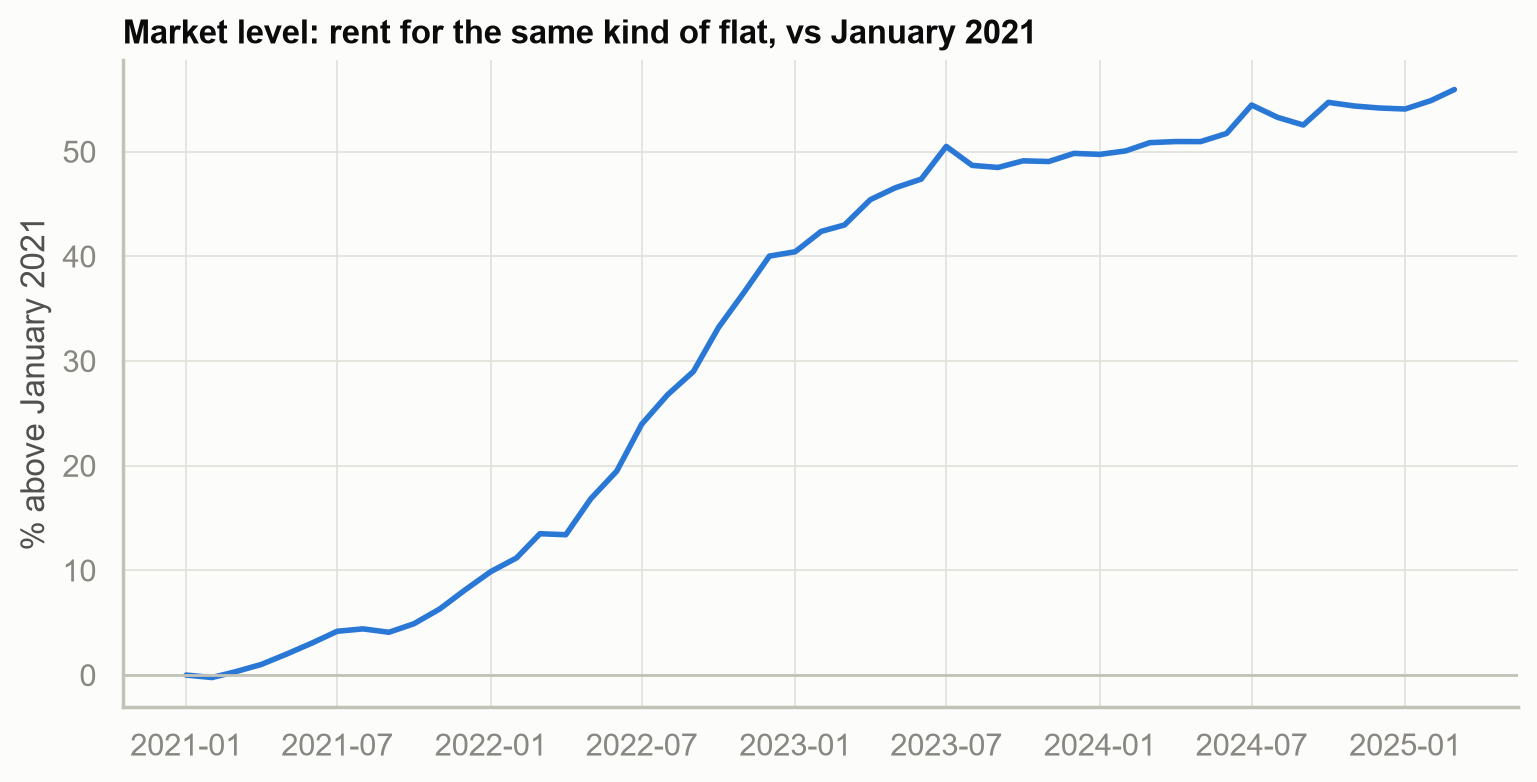
\includegraphics[width=\columnwidth]{figures/market_level.png}}
\caption{The market level: the hedonic index of rent for the same kind of flat, against January 2021.}
\label{fig:market-level}
\end{figure}

We therefore test whether the level should be forecast separately, by modelling
the rent of flat $i$ in month $t$ as
\begin{equation}
  y_{it} \approx L_t \times P_i ,
  \label{eq:level}
\end{equation}
a market level $L_t$ shared by all flats times the flat's premium $P_i$ over
it. The level is a hedonic index \cite{Rosen:1974:Hedonic}: the month
coefficients of a least-squares regression of log rent on month dummies, town,
flat type, flat model, floor area and flat age, so that it tracks the price of
the same kind of flat rather than which flats happened to rent. The tree learns
$y_{it}/L_t$ with no time feature, and a test prediction is
$\hat{P}_i \times \hat{L}_t$, with $\hat{L}_t$ forecast from training months
alone.

Four level forecasts were compared, each for a stated reason. \emph{Hold} repeats
the last training level. It is the control: it has the decomposition but no
trend, so it separates the effect of the split from the effect of a forecast.
\emph{Damped trend} \cite{Gardner:1985:Damped} continues the recent slope and
shrinks it each month, so the forecast bends toward flat. \emph{Straight line}
continues the average slope of the whole history, and we expect it to overshoot
because that slope includes the climb. \emph{Average} is the mean of hold and
damped trend, since averaged forecasts often beat their components when their
errors partly cancel \cite{Bates:1969:Combination}. An \emph{oracle} level,
fitted with the scored months' own rents, is a perfect level forecast but not a
perfect prediction: it still multiplies the tree's premiums. A method's distance
above it is approximately the cost of its level forecast.

An alternative to forecasting the level is to replace or supplement the month
index with series whose values are in the data for the test months: certificate
of entitlement (COE) prices, the auction price of the right to own a car, and
share indices for banks, property and the broad market. A share price with no
link to rent serves as a placebo control, so a macro series earns its place only
if it beats the placebo.

All comparisons use one holdout period (Section~\ref{sec:holdout}). That period
begins in a flat market, where hold, damped trend and average score within \$2 of
one another, so it cannot choose among them. Rolling-origin evaluation
\cite{Tashman:2000:OutOfSample} adds the climb: each month from December 2021 to
November 2023 serves in turn as the origin, the same model is retrained on months
up to it, and the next 16 months are scored.
